\section{Source code structure}

\subsection{Laravel Project Structure}
The following section describes the structure of the Laravel Project, meaning the structure of the source code for the back-end application.\\
Please note that this describes the structure of the code and only broadly the functionalities, for more information please refer to the rest of this document and to the comments associated with the source code, also more details about the standard structure of a Laravel project can be found in the \href{https://laravel.com/docs/5.5/structure}{official documentation}.

\subsubsection*{The App Directory}
\textbf{The app directory contains the core code of the application.}\\
The most important subdirectories in this folder are Http and Models.
\textit{Models} contain the classes comprising the application model.\\
\textit{Http} contains what is effectively the main application logic and has again several subfolders:
\begin{itemize}
	\item The \textit{Controllers} directory contains the classes that handle the methods binded to the endpoints.
	\item The \textit{Helpers} directory contains classes and scripts that provide functionalities used by the controllers.
	\item The \textit{Interfaces} directory contains classes that provide access to external services mentioned in section \ref{exservices}.
	\item The \textit{Middleware} directory contains the definition of HTTP filters that allow to filter the requests before or after such requests have been elaborated by the controllers.
\end{itemize}

\subsubsection*{The Bootstrap Directory}
The bootstrap directory contains the \textit{app.php} file which bootstraps the framework. This directory also houses a cache directory which contains framework generated files for performance optimization such as the route and services cache files.

\subsubsection*{The Config Directory}
The \textit{Config} directory contains all of the application's configuration files.

\subsubsection*{The Database Directory}
The \textit{Database} directory contains database migration and seeds. As we said in section \ref{dbmanagement}, Laravel uses the so-called database migrations in order to increase the portability of the application.\\
Each of the files found in the migrations defines a table in the database (see section \ref{dbmodel}) with an additional file that defines the relationships between them. 

\subsubsection*{The Public Directory}
The \textit{Public} directory contains the \textit{index.php} file, which is the entry point for all requests entering the application and configures autoloading. This directory also houses assets such as images, JavaScript, and CSS.\\
In our case it only contains the application Logo since there we do not use other resources.

\subsubsection*{The Resources Directory}
The \textit{Resources} directory contains views as well as raw, un-compiled assets such as LESS, SASS, or JavaScript. This directory also houses language files.\\
In the \textit{Views} subdirectory are the web files that contain the UI for the activation activation mail and confirmation page.

\subsubsection*{The Routes Directory}
The \textit{Routes} directory contains all of the route definitions for the application. By default, several route files are included with Laravel: \textit{web.php}, \textit{api.php}, \textit{console.php} and \textit{channels.php}.\\
The \textbf{web.php} file contains routes that are in the web middleware group, which provides session state, CSRF protection, and cookie encryption. The only route defined here is the one for the account activation endpoint since the rest of the functionalities are implemented via RESTful API.\\
The \textbf{api.php} file contains routes that are in the api middleware group, which provides rate limiting. These routes are intended to be stateless, so requests entering the application through these routes are intended to be authenticated via tokens and will not have access to session state. \\
This file defines all the routes for the implemented APIs.\\
The \textbf{console.php} file is where all Closure based console commands are defined. Each Closure is bound to a command instance allowing a simple approach to interacting with each command's IO methods. Even though this file does not define HTTP routes, it defines console based entry points (routes) into the application. Apart from Laravel default CLI commands we did not implemented any additional ones so no routes are defined here.\\
The \textbf{channels.php} file is where all of the supported event broadcasting channels are registered, again no additional routes are defined here.

\subsubsection*{The Storage Directory}
The \textit{Storage} directory contains compiled Blade templates, file based sessions, file caches, and other files generated by the framework. This directory is segregated into app, framework, and  logs directories. The app directory may be used to store any files generated by the application. The framework directory is used to store framework generated files and caches. Finally, the logs directory contains the application's log files.\\
The \textit{storage/app/public} directory may be used to store user-generated files.\\
Other than the framework generated files this folder is not used by our application.

\subsubsection*{The Tests Directory}
The \textit{Tests} directory contains automated tests. The \textit{Unit} subdirectory contains the Unit tests, while the \textit{Feature} subdirectory contains the Integration tests that verify the APIs functionalities.

\subsubsection*{The Vendor Directory}
The \textit{Vendor} directory contains the Composer dependencies.\\
Mainly the PHPUnit testing suite and Passport authentication package.

\subsection{Backend model description}
\label{dbmodel}
As we already said there is a tight correspondence between the Database Schema and the Model given the use of the ORM pattern.\\
The implemented structure of the Database and therefore of the various Models is depicted below.

\begin{figure}[H]
	\centering
	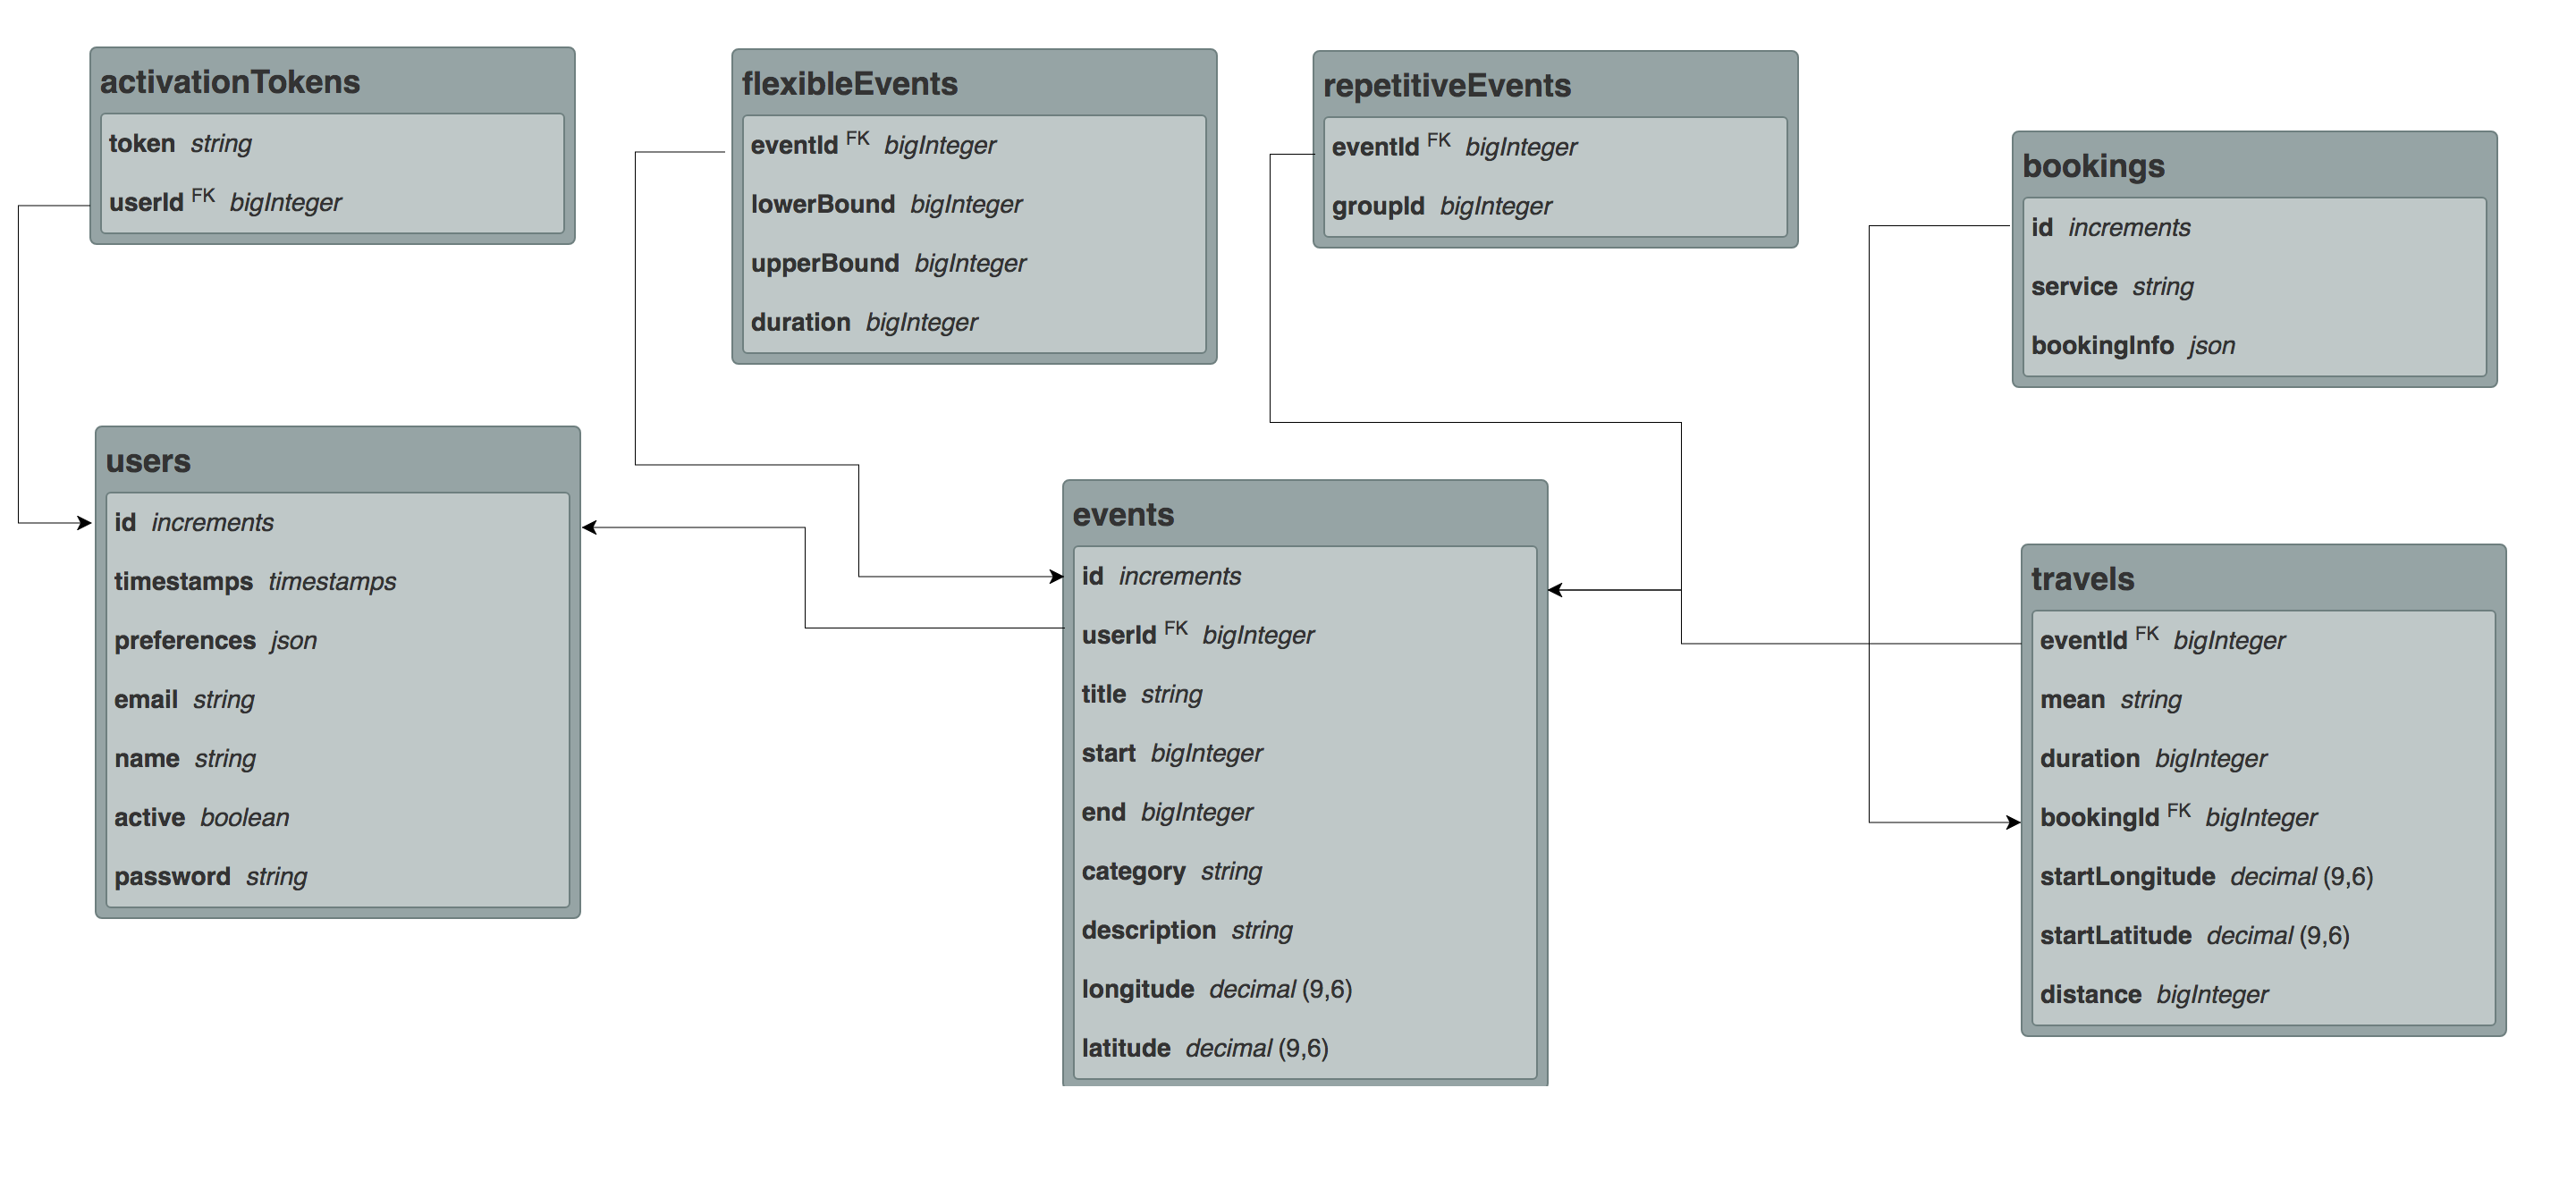
\includegraphics[scale=0.15]{DBModel}
	\caption{Model and Database Structure}
\end{figure}

\subsection{Xcode project structure}
The following section describes the structure of the Xcode Project, meaning the structure of the source code for the front-end iOS application.\\
Please note that this describes the structure of the code and only broadly the functionalities. For more details please refer to the source code comments and the \href{https://developer.apple.com/documentation/}{Xcode and iOS documentation}.
\\ \\
As we outlined in the previous section, view controllers are the foundation of our app’s internal structure. Each view controller manages a portion of your app’s user interface as well as the interactions between that interface and the model data. View controllers also facilitate transitions between different parts of your user interface. 
\\ \\
In order to make the code as clear and maintainable as possible, we organized files in different sections, according to their functionalities.

\subsubsection*{Model}
This section was intended to wrap all the relevant data structure useful to keep locally synchronized the data requested from the server. Classes have also supporting structure to help the JSON coding/decoding process. Model files are listed below:

\begin{itemize}
	\item \textit{User.swift}: this is the User model. It has a main struct User which encapsulates all the user-related information such as name, email, profile picture and the token to perform authenticated requests to the server. Furthermore, it contains structure to help the decoding of user credentials and owns the function which encapsulates the HTTP request to retrieve them.
	
	\item \textit{Preferences.swift}: this is the Preferences model. It has a main struct \textit{Preferences} which encapsulates all the user preferences for different travel means. It also contains support structures to help the coding/decoding process for the data sent/received to the server.
	
	\item \textit{Day.swift}: this is the day model. It holds all the day-related data such as the date of day currently selected by the user and the events list of the day. It also contains methods and structures to make easier the JSON coding/decoding and the string formatting.
	
	\item \textit{Event.swift}: this is the event model. It contains a main struct Event which is used for the coding/decoding of the JSON to send to or receive from the server. This structure contains all the event-related information, included the optional associated travel option. It also takes into account the current event selected in the \textit{DayViewController} and the list of associated travels.
	
	\item \textit{Booking.swift}: this is the booking model. It contains a main struct \textit{BookingInfo} which is used to encapsulate all the booking-related information received from the server. It also holds a global variable \textit{selectedBookingOption} which is used to store the currently available booking options retrieved from the server
\end{itemize}

\subsubsection*{Log View Controllers}
All the view controllers related with user authentication and sign up process.
\begin{itemize}
	\item \textit{LogViewController.swift}: it is the initial view controller. It handles the log in process sending an authentication request to the server. In case of success moves to the \textit{DayViewController}.
	\item \textit{SignUpViewController.swift}: displays the registration form and, in case of success, segues to \textit{StartViewController}.
	\item \textit{StartViewController.swift}: shows to the user that a confirmation email has been sent to his/her account and let go back to the \textit{LogViewController} for the authentication.
\end{itemize} 

\subsubsection*{Side Menu View Controllers}
Gathers all the files that generate the left side menu, including the Objective-C \textit{SWRevealViewController} external library.
\begin{itemize}
	\item \textit{MenuViewController.swift}: displays the slide out left side menu and the relative options.
	\item \textit{MenuTableViewCell.swift}: represents a cell of the menu.
	\item \textit{SWRevealViewController.h}: header file of the library.
		\item \textit{SWRevealViewController.m}: source file of the library.
\end{itemize}

\subsubsection*{Navigation View Controllers}
This section contains all and only the view controllers reachable from the left-side menu.
\begin{itemize}
	\item \textit{DayViewController.swift}: this is the "home" of the application. It is the first view displayed after the log in, showing the current date and the associated events, organized in a scrollable view. Every time the view is loaded, it performs an HTTP GET request to retrieve the events of the day.\\
	On the top-right corner it has an add button that leads to the \textit{AddEventViewController}. Furthermore, if the user taps on an event, a view with detailed information will be displayed.
	\item \textit{CalendarViewController.swift}: shows an horizontally scrollable calendar, marking the current day in red and each day with at least one event with a dot. If a day cell in the calendar is tapped, the \textit{DayViewController} will be displayed, showing the events of the selected day, if present.
	\item \textit{PreferencesViewController.swift}: displays a scrollable view to set/edit travel means preferences. On the top, means can be globally activate/deactivate through toggle buttons.
	The save button in the right corner embeds all the infos in a JSON file and send it to the server to save the preferences.
	\item \textit{SettingsViewController.swift}: within this view, users can edit their profile picture, their name and change their password or email.
	\item \textit{CreditsViewController.swift}: displays the credits of the application, showing the \textit{Politecnico di Milano} logo and the developers' name.
\end{itemize}

\subsubsection*{Event-related View Controllers}
This section embeds all the view controllers connected with event management.
\begin{itemize}
	\item \textit{AddEventViewController.swift}: handles the creation of an event, displaying a form to fill with all the necessary information, included the location of the event (handled separately from the \textit{LocalSearchViewController}) and an eventually travel option.
	When the top-right "Done" button is tapped, an HTTP POST request is sent to the server.
	\item \textit{TravelViewController.swift}: handles the retrieve of the possible travel option of an event from the server and displays them in a scrollable view.
\end{itemize}

\subsubsection*{Booking View Controllers}
All the view controllers involved in the booking process of third-party services.
\begin{itemize}
	\item \textit{BookingViewController.swift}: it currently handles the Uber booking functionalities. At the top it displays the Uber sign in button that leads to the Uber app in order to authenticate the user.
\end{itemize}

\subsubsection*{Settings View Controllers}
Gathers all the view controllers reachable from the \textit{SettingsViewController}.
\begin{itemize}
	\item \textit{ChangePasswordViewController.swift}: handles the change password process. Shows two text field for the old and the new password and has a "save" button to send the information to the server. 
\end{itemize}

\subsubsection*{Cells Table Views}
In this section are gathered all the files that represent a dynamic cell in a table view controller.
\begin{itemize}
	\item \textit{EventCell.swift}: is a cell of the event table view in the \textit{DayViewController}. It shows the title, the description and when the event takes places. It also has two icons: one for the travel mean associated, one for the booking option.
	\item \textit{CalendarCell.swift}: is a cell of the calendar collection view in the \textit{CalendarViewController}. It shows the number of the corresponding day and a bullet if the day contains at least one event.
	\item \textit{TravelCell.swift}: is a cell that represents a travel option in the \textit{TravelViewController}. It displays the mean, the duration and the distance. 
	\item \textit{BookingCell.swift}: is a cell that represents a booking option in the \textit{BookingViewController}. It shows the type of mean, the duration, the distance and the price.
\end{itemize}

\subsubsection*{Location View Controllers}
These are all the view controllers connected with the location menagment.
\begin{itemize}
	\item \textit{LocalSearchViewController.swift}: displays a view of the map through the Apple MapKit and provides a search bar to seek locations.
	\item \textit{LocationSearchTableViewController.swift}: overlapping table view which shows the places that match the request.
\end{itemize}

\subsubsection*{Supporting files}
\begin{itemize}
	\item \textit{Main.storyboard}: a visual representation of the user interface of the application, showing screens of content and the connections between those screens.
	\item \textit{Info.plist}: is a structured text file that contains essential configuration information for a bundled executable.
	\item \textit{AppDelegate.swift}: its in charge of the application life cycle. Providing a starting point, delegating what to do when the app is put in the background, reactivated, or being terminated, and responds to events that target the app itself rather than specific view.
	\item \textit{Podfile.txt}: is a specification that describes the dependencies of the targets of the Xcode project.
\end{itemize}

\subsection{Frontend model description}
\begin{figure}[H]
	\centering
	\makebox[\textwidth][c]{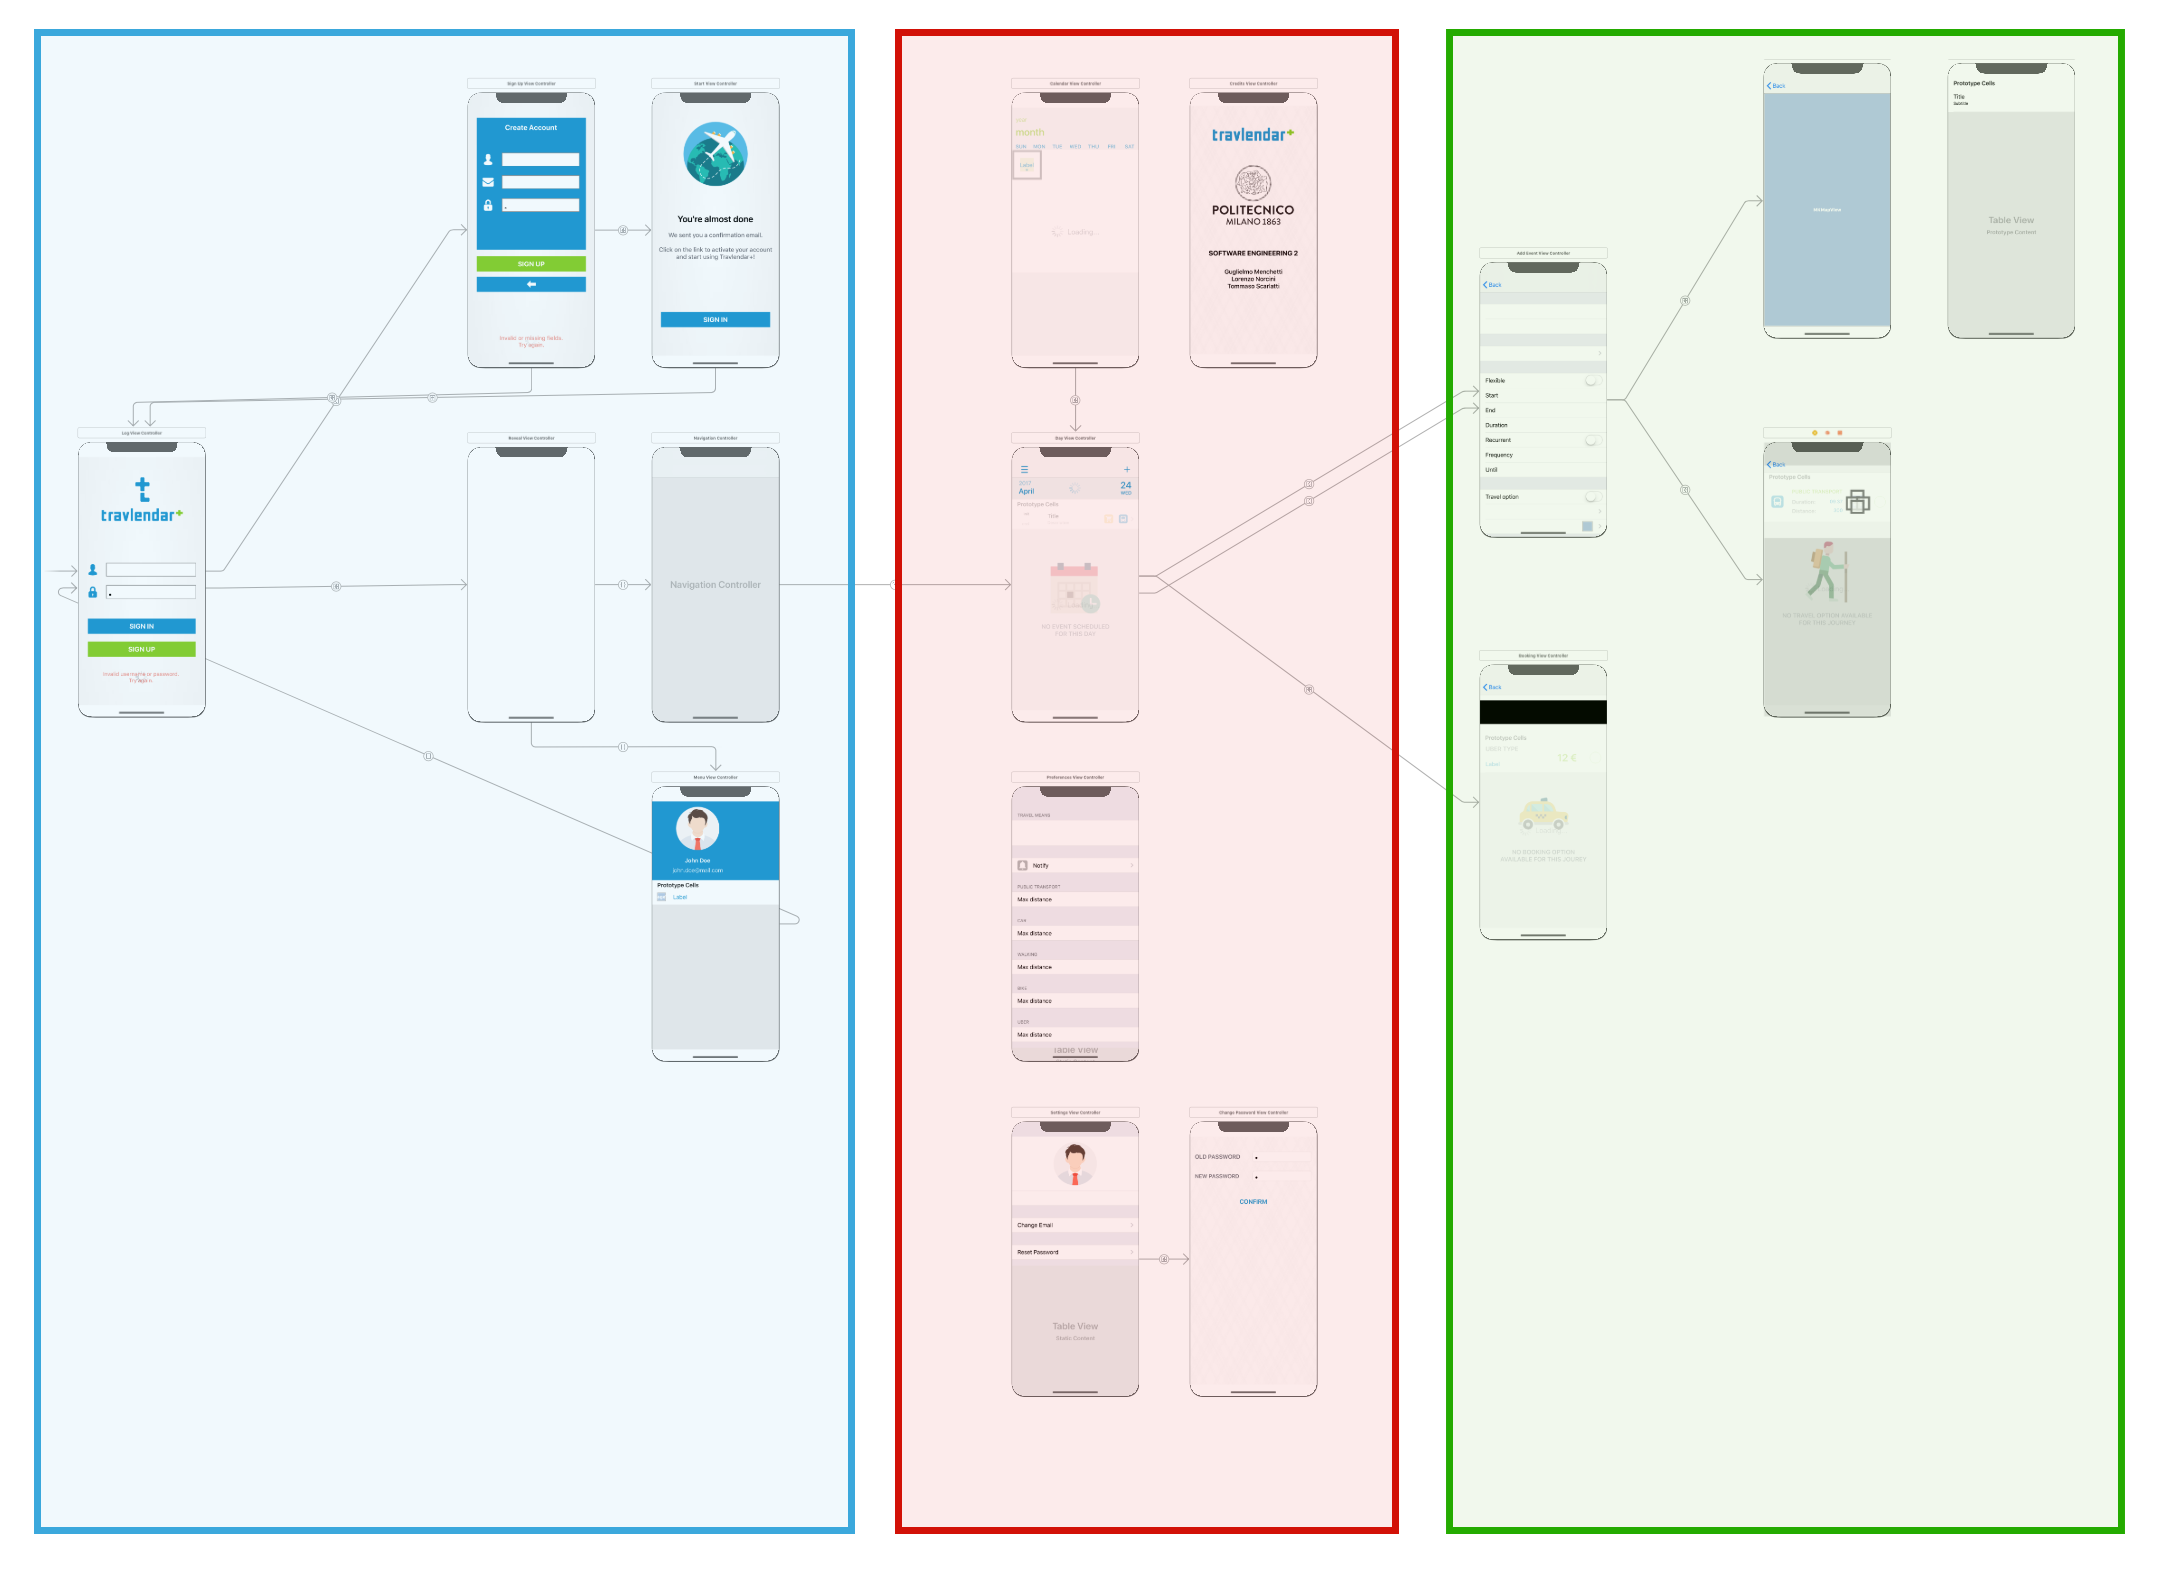
\includegraphics[width=1.2\textwidth]{storyboard}}%
	\caption{Storyboard structure}
\end{figure}

The above figure shows an overall view of the Main.storyboard file. Here we can clearly see the distinct sections of the application and the connections between them.
\\ \\
For clarity reasons, view controllers have been divided into three different logic categories.

\begin{itemize}
	\item \textbf{Authentication, Registration and Side Menu} (blue)\\
	In this category we have all the view controllers related with authentication and registration process and those responsible for the appearance of the slide-out left side menu.\\
	They are the entry point of the application.  Each new user must pass first from the \textit{SignUpViewController}, then to the \textit{LogInViewController} and finally to the \textit{MenuViewController} to navigate into the application.
	 
	\item \textbf{Navigation} (red)\\
	This category contains all and only the view controllers reachable from the left-side menu.
	
	\item \textbf{Event-related} (green)\\
	All the view controllers reachable from the \textit{DayViewController}. They are all related with the creation or the modification of an event.
\end{itemize}

\subsubsection*{Screenshots}
For each category we show here a bunch of screenshots of the application.
\begin{figure}[H]
	\centering
	\begin{subfigure}{0.25\textwidth}
		\centering
		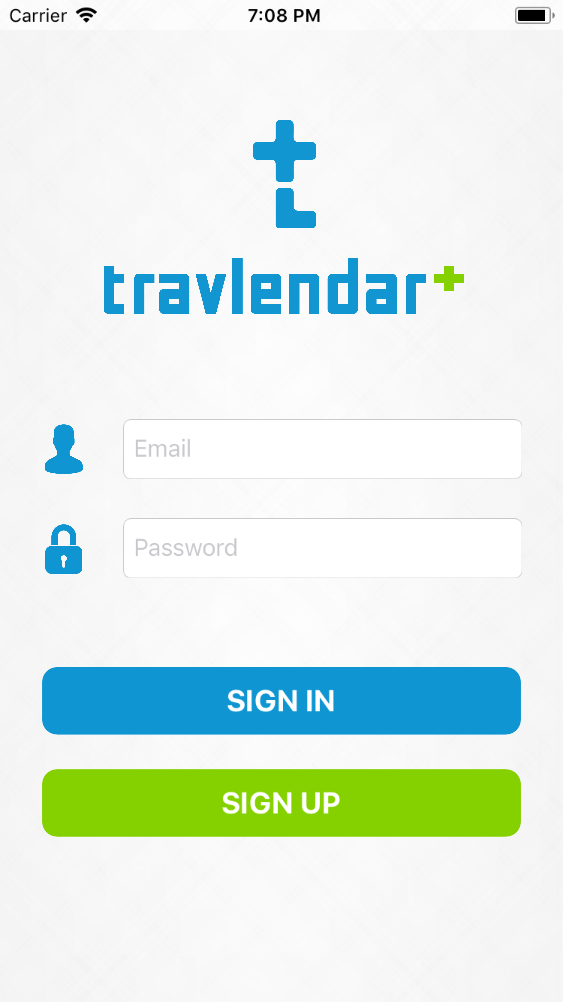
\includegraphics[width=\textwidth]{login.png}
	\end{subfigure}
	~
	\begin{subfigure}{0.25\textwidth}
		\centering
		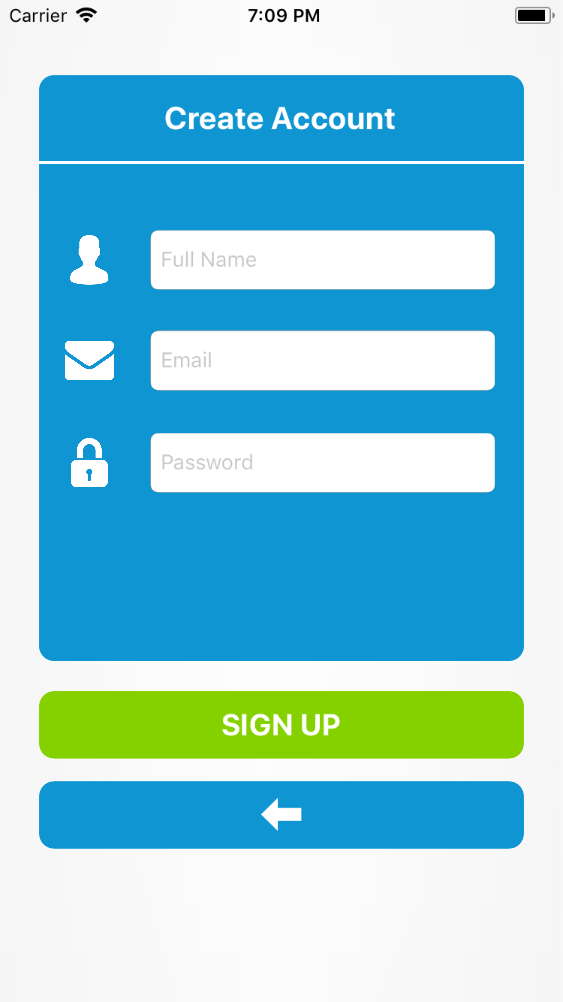
\includegraphics[width=\textwidth]{signup.png}
	\end{subfigure}
	~
	\begin{subfigure}{0.25\textwidth}
		\centering
		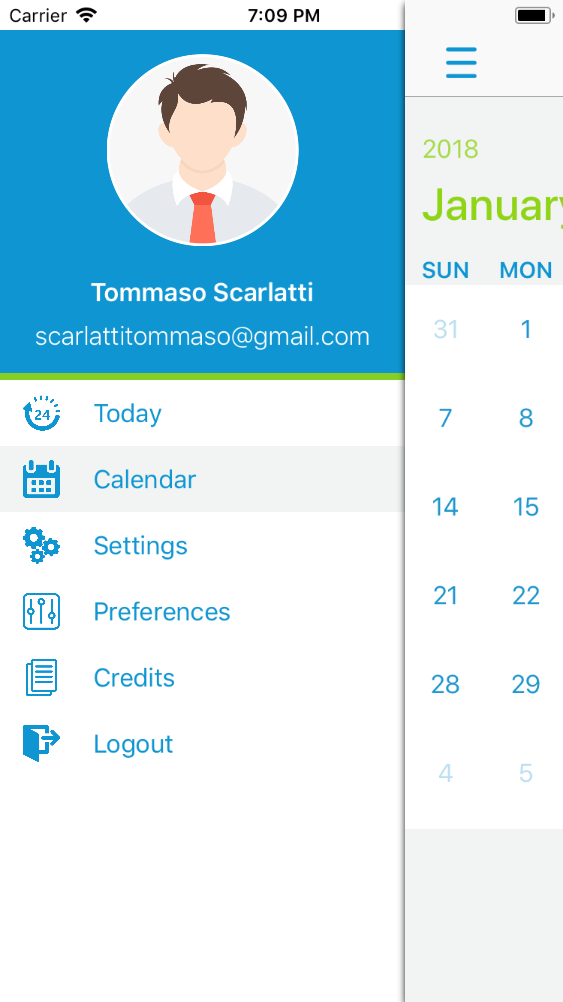
\includegraphics[width=\textwidth]{menu.png}
	\end{subfigure}
	\caption{Authentication, Registration and Side Menu}
\end{figure}


\begin{figure}[H]
	\centering
	\begin{subfigure}{0.25\textwidth}
		\centering
		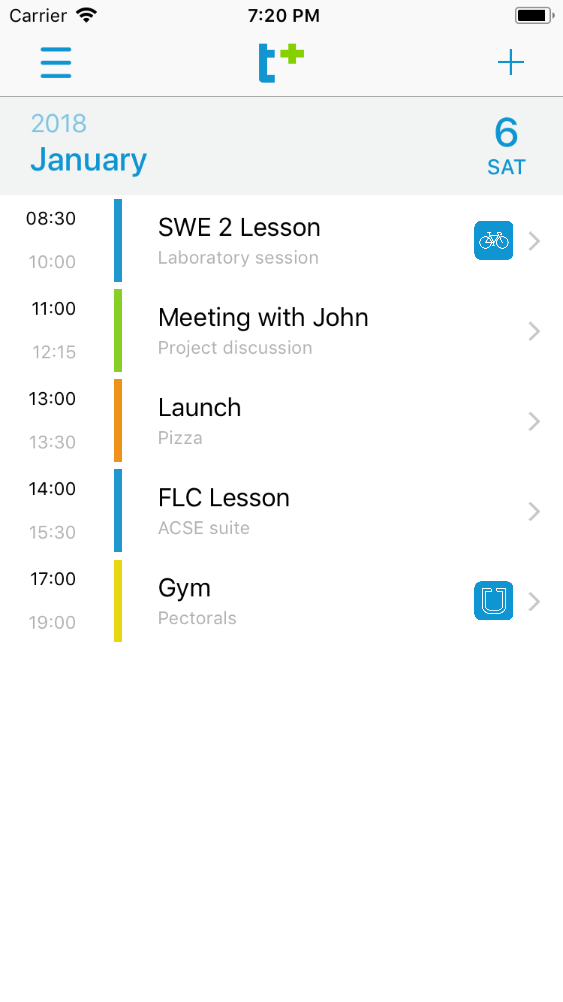
\includegraphics[width=\textwidth]{day.png}
	\end{subfigure}
	~
	\begin{subfigure}{0.25\textwidth}
		\centering
		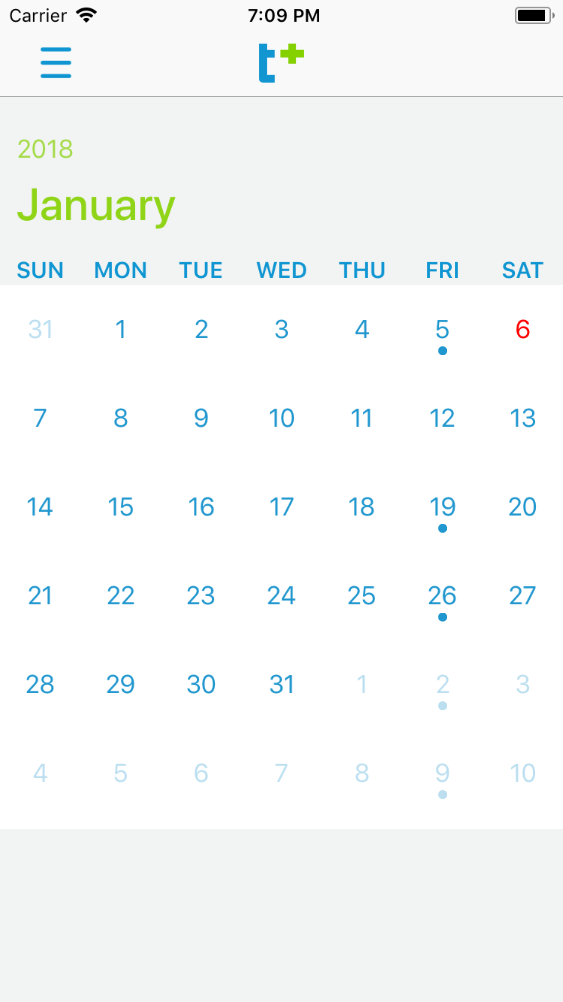
\includegraphics[width=\textwidth]{calendar.png}
	\end{subfigure}
	~
	\begin{subfigure}{0.25\textwidth}
		\centering
		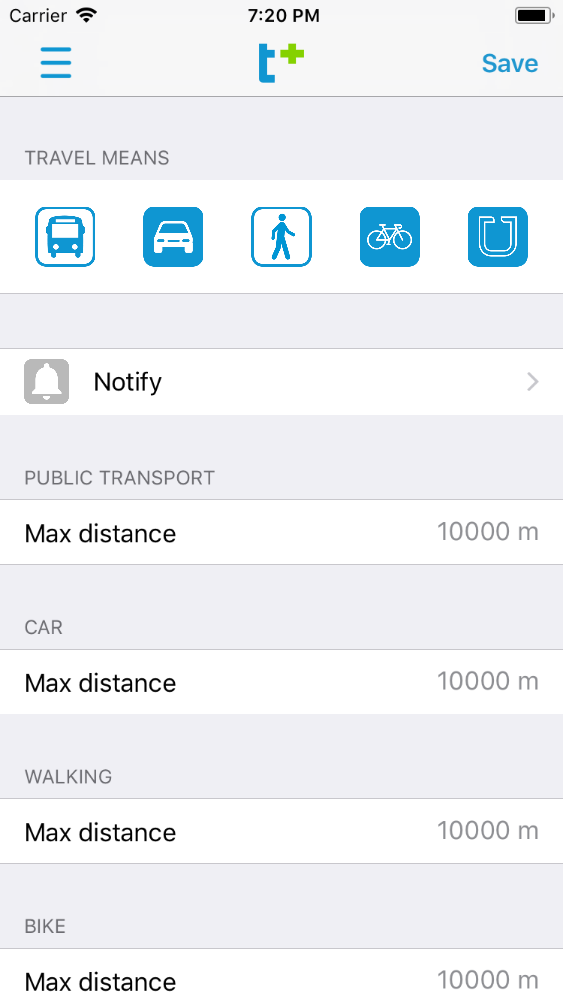
\includegraphics[width=\textwidth]{preferences.png}
	\end{subfigure}
	~
	\begin{subfigure}{0.25\textwidth}
		\centering
		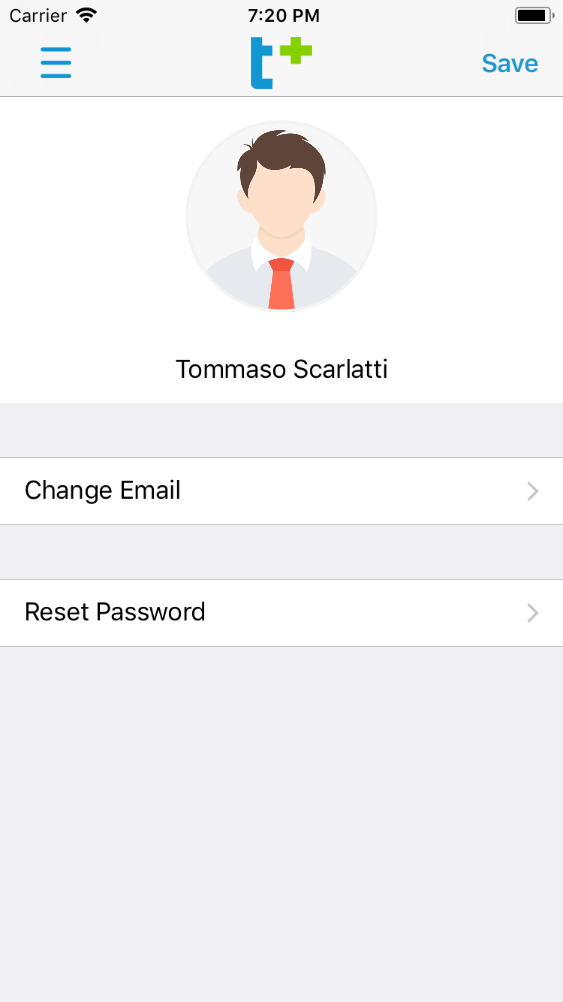
\includegraphics[width=\textwidth]{settings.png}
	\end{subfigure}
	~
	\begin{subfigure}{0.25\textwidth}
		\centering
		
\includegraphics[width=\textwidth]{credits.png}
	\end{subfigure}

	\caption{Navigation View Controllers}
\end{figure}

\begin{figure}[H]
	\centering
	\begin{subfigure}{0.25\textwidth}
		\centering
		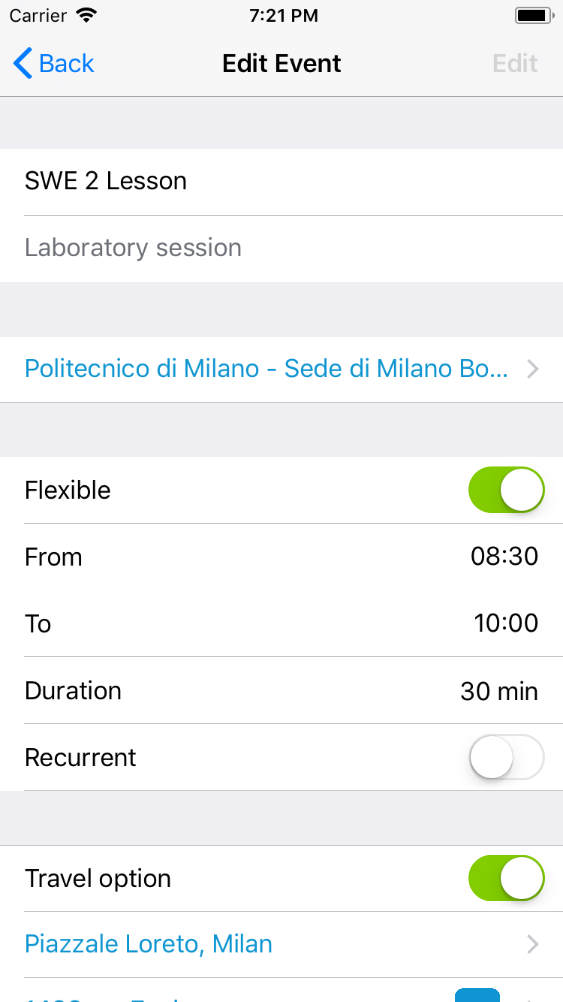
\includegraphics[width=\textwidth]{event.png}
	\end{subfigure}
	~
	\begin{subfigure}{0.25\textwidth}
		\centering
		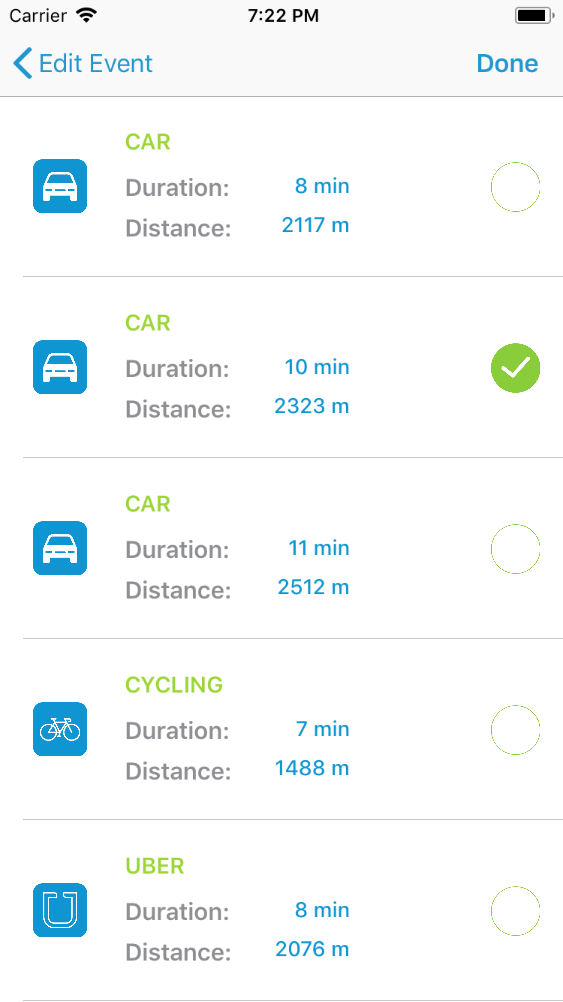
\includegraphics[width=\textwidth]{travel.png}
	\end{subfigure}
	~
	\begin{subfigure}{0.25\textwidth}
		\centering
		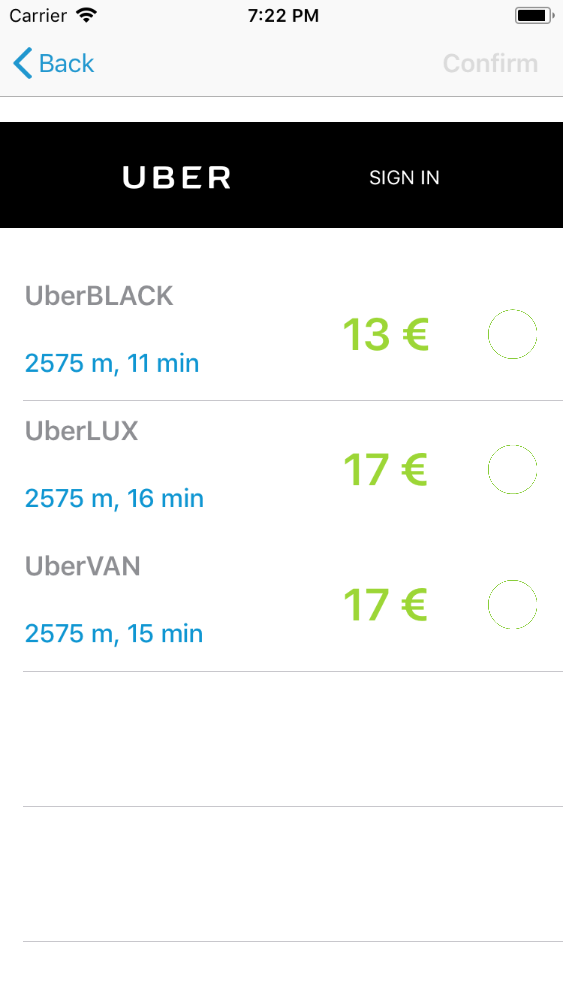
\includegraphics[width=\textwidth]{uber.png}
	\end{subfigure}
	\caption{Event-related View Controllers}
\end{figure}
